\documentclass[12pt]{amsart}
\usepackage{geometry} % see geometry.pdf on how to lay out the page. There's lots.
\geometry{a4paper} % or letter or a5paper or ... etc
% \geometry{landscape} % rotated page geometry
\usepackage{url}
%\usepackage{tocloft}

\usepackage{tikz}
\usetikzlibrary{positioning}
\usetikzlibrary{arrows.meta}
\tikzset{>={Latex[width=3mm,length=3mm]}}

\newcommand{\AM}{\mathbf{A}}
\newcommand{\BM}{\mathbf{B}}
\newcommand{\CM}{\mathbf{C}}
\newcommand{\DM}{\mathbf{D}}
\newcommand{\IM}{\mathbf{IQ}}
\newcommand{\KM}{\mathbf{K}}

\newcommand{\R}{\mathbb{R}}

\newcommand{\xv}{\mathbf{x}}

\title{Manual: dev4 for LLRF for AWAKE2}
\author{Kristiaan Pelckmans, April 2024}
\date{} % delete this line to display the current date

%%% BEGIN DOCUMENT
\begin{document}

\maketitle

\begin{abstract}
A manual for the  of the Low Level Radio Frequency (LLRF) development for AWAKE2 in Uppsala University.

\vspace{+25mm}


\centering\includegraphics[width=1in]{im/dev4.png} 


\vspace{+25mm}


%{\em This is a living document, reflecting the state of development as of April 2024.}

\end{abstract}

\newpage
\tableofcontents
\newpage

%\addtocontents{toc}{\protect\mbox{}\protect\hrulefill\par}
\section{Introduction}
%%%%%%%%%%%

This document describes the development of a low level RF (LLRF) control system
for exploratory use with a micro Telecommunication Computing Architecture (MicroTCA.4) platform
in the AWAKE2 (run C) experiment.

The present assignment is to make a working LLRF  embedded system in the MicroTCA crate, using traditional tools as PID control and IQ sampling.
There are plenty of opportunities for further research, summarised in conclusions.
Key challenge in this assignment was not so much conceptual,
but to get acquainted and constructive with the nitty gritty details of the embedded system implementation.

\subsection{MicroTCA4.0}

MicroTCA.4 is a platform for embedded system programming, specially designed to address the needs in large physics experiments.
MicroTCA is based on advanced TCA for implementing active embedded systems, often used in the telecommunication or military industry.
Presently, implementations of LLRF systems based on the outdated VME or PXI standard  are upgraded to MicroTCA,
with new developments increasingly often realised natively in MicroTCA4.0.


\subsection{AWAKE 2C}

AWAKE is a collaboration project \footnote{ See \url{https://home.cern/science/accelerators/awake}} at CERN
aiming to proof feasibility of wakefield acceleration.
In AWAKE, a plasma wakefield is driven by a high-energy proton bunch (400 GeV, length 6-8 cm, or 19kJ per bunch, Adli et al., 2018).
This wakefield is then used to accelerate electrons to 2 GeV, aiming for levels of up to 200 GeV. 
Wakefield acceleration may provide a 100 fold increase of gradient (i.e. 10GV/m rather than 0.1 GV/m) as compared to standard RF acceleration techniques.
The proton bunch is delivered by the Super Proton Synchrotron (SPS) at CERN, delivering beam in 'only' a few percent of the cycles.
The plasmas operate in a constant temperature of 200C, and an ambient atmosphere of Xenon.
Figure (\ref{fig:regime}) displays the energy regime where the AWAKE technology is of relevance.
\begin{figure}[htbp] %  figure placement: here, top, bottom, or page
   \centering
   \includegraphics[width=5in]{im/awake_regime.png} 
	\caption{Regimes (energy levels) that AWAKE can prompt, as compared to other machines.
	This graph displays particularly the regime of mixing strength versus dark photon mass.
	[84] Alemany, R.; Alemany, R.; Burrage, C.; Bartosik, H.; Bernhard, J.; Boyd, J.; Brugger, M. 
	Summary Report of Physics Beyond Colliders at CERN. arXiv 2019, arXiv:1902.00260.}
   \label{fig:regime}
\end{figure}

\begin{figure}[htbp] %  figure placement: here, top, bottom, or page
   \centering
   \includegraphics[width=5in]{im/awake2.png} 
   \caption{\em Overall layout of the AWAKE2 (Run C) experiment with both plasma fields.}
   \label{fig:run2c1}
\end{figure}

The first iteration of AWAKE has shown promising result based on a 10 meter single plasma (Acc'or) field for realising a wakefield (Adli et al., 2018).
Run 2C (see Figure \ref{fig:run2c1}) introduces a 2e plasma field (tube of 10cm $\times$10m on the beam line) 
preceding (by about 10cm) the accelerating plasma field order to increase efficiency further.
This (self-modulating) plasma field is used to pre-seed the wakefield.
%\begin{figure}[htbp] %  figure placement: here, top, bottom, or page
%   \centering
%   \includegraphics[width=5in]{im/run2c.png} 
%   \caption{\em Overall layout of the AWAKE2 (Run C) experiment with both plasma fields: 
%   (1) Self Modulated plasma field (SM'or) driven by proton bunches from the SPS, and 
%   (2) the actual accelerator plasma field (Acc'or) of electrons.
%   This work focuses on the LLRF for the electron LINAC feeding the SM'or (green line).}
%   \label{fig:run2c}
%\end{figure}



 \subsection{A second e- LINAC}

\begin{figure}[htbp] %  figure placement: here, top, bottom, or page
   \centering
   \includegraphics[width=5in]{im/esys2.png} 
   \caption{\em Schematic overview of the 2 electron injector lines to be controlled.}
   \label{fig:elinac}
\end{figure}

 
\begin{figure}[htbp] %  figure placement: here, top, bottom, or page
   \centering
   \includegraphics[height=1.6in]{im/layout1e.png} 
   \includegraphics[height=1.6in]{im/layout2e.png} 
   \caption{\em The two electron injector lines (needed for AWAKE run 2C.
   	Left panel : 1e injector line with S-band e-gun and a single S-band RF accelerating structure,
   	Right panel : 2e injector line with S-band e-gun, an X-band buncher and two X-band RF accelerating structures.
    }
   \label{fig:elinac}
\end{figure}


Figure \ref{fig:elinac} displays the new electron (e-) LINAC needed in AWAKE 2C for driving the self modulating (SM) plasma field.
Such LINAC is equipped with an electron gun, a buncher and two RF accelerator structures.
Each of these is properly controlled by an RF line.
Figure (\ref{fig:run2c.egun}) displays a typical electron gun as used in AWAKE.
\begin{figure}[htbp] %  figure placement: here, top, bottom, or page
   \centering
   \includegraphics[width=5in]{im/egun.png} 
   \includegraphics[width=5in]{im/eacc.png} 
   \caption{\em  (top panel) a schematic overview of an electron gun.
   			(bottom panel) a schematic overview of a bunching and acceleration structure.
			}
   \label{fig:run2c.egun}
\end{figure}
Operation of this 2e plasma requires a new electron line to be developed.


Both e-guns operate in S band.
The first electron injector line needs an added S band RF.
The second electron injector line needs 2 added X band controllers.
The x-band technology is an up-converted version of the S-band developments.
This totals 5 RF structures that need to be controlled RF supply and measurement points.
A schematic overview of a control loop is shown in Figure (\ref{fig:loop2023}).
The layout of the first control loop is displayed in Figure (\ref{fig:loop1}).

The components are described as follows:
\begin{itemize}
\item[SSPA:] The Solid State Power Amplifier has as input signal the result of the VM, and amplifies this to 200W (roughly 55dB). 
\item[Klystron:] The Pulse Modulator and Klystron amplifies this 200W signal to peak powers of 7.5MW.
\item[PC:] The BOC Pulse Compressor (PC) compresses the pulse with a factor 6, resulting in a peak of 15MW.
\item[Acc'or:] The RF structure accelerating the electrons before injecting in the main beam.
\end{itemize}

\begin{figure}[htbp] %  figure placement: here, top, bottom, or page
   \centering
   \includegraphics[width=5in]{im/loop2023.png} 
   \caption{\em Schematic overview of a feedback loop in this context.
   	Note that the data acquisition 'only' acts as an observer.}
   \label{fig:loop2023}
\end{figure}



\begin{figure}[htbp] %  figure placement: here, top, bottom, or page
   \centering
   \includegraphics[width=5in]{im/loop1.png} 
   \caption{\em 
   	Layout of the present control loop, with BCs as connected to the MicroTCA crate (names of BC as used in the above figure marked in red).
	The PID SISO loop focusses on the VM (as input signal) and BC1.fwd (Channel 1, as output signal).}
   \label{fig:loop1}
\end{figure}


\begin{figure}[htbp] %  figure placement: here, top, bottom, or page
   \centering
   \includegraphics[width=4in]{im/pulse.png} 
   \includegraphics[width=5in]{im/pulseP2.png} 
   \caption{\em Schematic of a pulse, occuring at 10Hz: 
   (a) (from O.Troeng, 2017) with adjusted time lengths. The Y-axes denote power (Watt). 
   (b) the layout of a pulse (blue square) in terms of the $I$ and $Q$ signals, with triggers from the interlock.}
   \label{fig:pulse}
\end{figure}


\subsection{Requirements}
%%%%%%%%%%%%%%

The desired stability properties (i.e. phase and amplitude coherence) are summarised in Table (\ref{tab:table1}).
Process stability of the closed control loop is a given. Stability in this table refers to pulse-to-pulse variation, and is more commonly referred 
as amplitude/phase coherence.
The ultimate aim is to synchronise the electron bunches exactly with the wakefield, requiring tight (actively controlled) phase coherence
of the feeding RF fields.
\begin{table}
  \begin{center}
    \caption{Desired stability properties.}
    \label{tab:table1}
    \begin{tabular}{|l || c|r|} % <-- Alignments: 1st column left, 2nd middle and 3rd right, with vertical lines in between
      \hline
      \textbf{Property} & \textbf{S-band} & \textbf{X-band}\\
      \hline
          Operating freq. 	& 2.997899068GHz 	& 11.991596272GHz  \\
          Pulse length 		& 6 us 			& 100-1500 ns \\
          Bandwidth 		& $>$20 MHz 		& $>$20 MHz \\
          Pulse repetition rate	& 9.97 Hz			& 9.97 Hz \\
          % $\sharp$ signals DAQ		& 14+Ref 	& 14+Ref \\
          % $\sharp$ signals generated & 2		& 2 \\
         Jitter (difference timing-pulse start)		& $<$ 30 fs	& $<$30 fs \\
          Amplitude stability		& $10^{-4}$ 	& $10^{-4}$ \\
          \hline
    \end{tabular}
  \end{center}
\end{table}




\subsection{Disturbances}

This subsection gives an overview of the disturbances on the present signals.
\begin{itemize}
\item[MICROPHONICS:] The effect of external mechanical vibrations account for the bulk of measured disturbances.
\item[DROOP] The performance of the active hardware as the klystron declines over time.
\item[RIPPLE] External effects tend to induce ripple in the desired signals:
	external effects will be compensated for when consistent.   
\item[BEAM] The loading of the beam induces a disturbance of the field. This effect is insignificant in the setup of AWAKE.
\item[POWER] The supply of power induces significant variations.
\item[THERMAL] Variations in the outside temperature imply a significant disturbance effect. 
\item[DUTY] Variations into the duty cycle induce a significant disturbance effect.  
\item[JITTER ] Clock jitter in the ADC clocks is impacting directly the measurement accuracy.
	The manual of the AD9510 PLL chips indicate a 40 fs jitter.
\item[X-talk] One has considerable cross-talk between the different channels, especially if the MicroTCA powers more SIS+RTM pairs.
\item[AE] Ambient (environmental) electronic radiation is a source of noise in the ADC. 
\end{itemize} 


\subsection{Pulse compressors}

Figure (\ref{fig:pc}) illustrates the effect of a SLED Pulse Compressor (PC).
The result of a BOC pulse compressor is similar, only needing a single cavity 
(see \url{3 GHz Barrel Open Cavity (BOC) RF pulse compressor for CTF3}).
CERN has developed a SLED-I pulse compressor for use in X-band (see Woolley, Syratchev, Dexter, 2017), and figured a PI
pulse-to-pulse approach to give the pulse from the compressor a flat top.
The S-band will use a BOC, and the X-band setup a SLED-I.

\begin{figure}[htbp] %  figure placement: here, top, bottom, or page
   \centering
   \includegraphics[width=3in]{im/boc.png} \\
   \includegraphics[width=1.5in]{im/Boc_Sband.jpg} 
   \includegraphics[width=1.5in]{im/Sled_Xband.jpg} 
   \caption{\em  (a) The behavior of the SLED pulse compressor (Z.D. Farkas et al., 1974).
   	(b) Photo of the BOC pulse compressor to be used in the first electron injector line,
	(c) Photo of the SLED-I pulse compressor to be used in the second electron injector line.    }
   \label{fig:pc}
\end{figure}

%
%\begin{figure}[htbp] %  figure placement: here, top, bottom, or page
%   \centering
%   \includegraphics[width=2in]{sin.png} 
%   \includegraphics[width=2in]{sin2.png} 
%   \includegraphics[width=2in]{sin3.png} 
%   \includegraphics[width=2in]{sin4.png} 
%   \caption{}
%   \label{fig:sin}
%\end{figure}
%

\begin{center}
    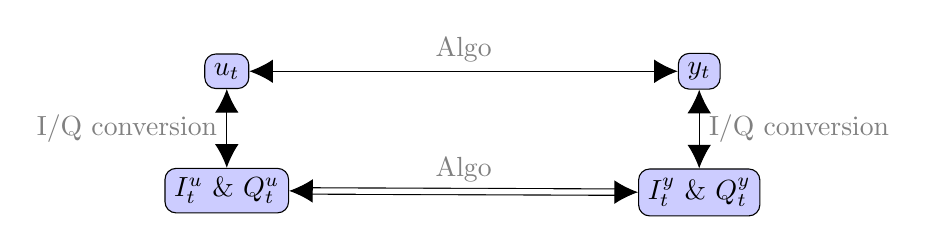
\begin{tikzpicture}
    \node (u) at (0,4) [draw, rounded corners, fill=blue!20] {$u_t$};
    \node (uiq) [draw, rounded corners, fill=blue!20, below=of u] {$I_t^u$ \& $Q_t^u$};
    \node (y) at (6,4) [draw, rounded corners, fill=blue!20] {$y_t$};
    \node (yiq) [draw, rounded corners, fill=blue!20, below=of y] {$I_t^y$ \& $Q_t^y$};
    
    \path [draw, <->] (u) -- node [above, color=gray] {Algo } (y);
    \path [draw, <->,double distance=1.9pt] (uiq) -- node [above, color=gray] {Algo} (yiq);
    \path [draw, <->] (u) -- node [left, color=gray] {I/Q conversion} (uiq);
    \path [draw, <->] (y) -- node [right, color=gray] {I/Q conversion} (yiq);
    \end{tikzpicture}
\end{center}



\newpage
\addtocontents{toc}{\protect\mbox{}\protect\hrulefill\par}
\section{LLRF Hardware}
%%%%%%%%%%%

\subsection{Setup}


The hardware consists of:
\begin{itemize}
\item Workstation (running centOS), with a licensed Vivado 2020.1 running.
\item MicroTCA (micro telecommunication Computing Architecture)  crate.
\item R\&S signal generator devices, serving LO, reference and clock signal.
\item An internet router, connecting all hardware modules.
\end{itemize}

\begin{figure}[htbp] %  figure placement: here, top, bottom, or page
   \centering
   \includegraphics[width=5in]{im/pc.png} 
   \caption{\em Hardware setup.}
   \label{fig:pc}
\end{figure}
The setup of the workstation/crate/router/signal generators
is displayed in (\ref{fig:pc}).
The MicroTCA crate has the following components on board:
\begin{itemize}
\item Crate (Schroff 19”, 19U crate, with vertical cooling).
\item N.A.T.-MCH (-PHYS80) (with CLK module and PCIe switch).
\item N.A.T.-MCH-RTM (-BM) (with E3 COMex based on a Xeon processor, running Ubuntu 20.04 TLS).
\item 2 N.A.T. power units (600 W).
\item Backplane (TCLKA, TCLKB).
\item RF-backplane, distributing power for the RF-backplane, CLK, REF and LO to all the RTMs connected to the RF-backplane.
\item 2 pairs of SIS8300KU+DWC8VM1 AMC cards (on slot 8 and slot 11 respectively)
\item A NAMC - PMC module (NAMC-PMC-T261-20R).
\end{itemize}
The workstation runs vivado 2020.1, and is connected to the NAT-MCH via telnet
\begin{verbatim}
> telnet 192.168.30.50
\end{verbatim} 
and to the COMex via a secure shell (SSH):
\begin{verbatim}
> ssh -X mch@192.168.30.105
\end{verbatim} 
The RF-backplane provides functionality to distribute LO, REF and clock signals to all the RTM cards connected to the RF-backplane.
Fotos from the MicroTCA crate (as of 20 Aug. 2022) are displayed in figure (\ref{fig:foto}).
The signals to be provided at the frontplate of the SIS, and the RTM are specified in Figures (\ref{fig:card}) and Figure (\ref{fig:fp}).
\begin{figure}[htbp] %  figure placement: here, top, bottom, or page
   \centering
   \includegraphics[height=2.5in]{im/foto_front.jpg}
   \includegraphics[height=2.5in]{im/foto_rtm.jpg} 
   \caption{\em Foto's of the MicroTCA crate 
   	(a) front side of the MicroTCA crate (with the 2 SIS 8300KU digitiser AMCs),
	(b) rear side of the MicroTCA crate (with the 2 RTMs (DWC8VM1) cards).}
   \label{fig:foto}
\end{figure}


\begin{figure}[htbp] %  figure placement: here, top, bottom, or page
   \centering
   \includegraphics[height=1.6in]{im/sis.png} 
   \includegraphics[height=1.6in]{im/rtm.png} 
   \caption{\em Schematic of (a) the SIS8300KU AMC and (b) the DWC8VM1 RTM card.}
   \label{fig:card}
\end{figure}
 


\begin{figure}[htbp] %  figure placement: here, top, bottom, or page
   \centering
   \includegraphics[height=4in]{im/RTM_fp_signals.jpeg}
   \caption{\em Signal specifications as to be provided on the frontplate of the RTM (courtesy Struck manual, 2023).}
   \label{fig:fp}
\end{figure}

\begin{figure}[htbp] %  figure placement: here, top, bottom, or page
   \centering
   \includegraphics[height=2in]{im/RFbackplane.png}
   \caption{\em Backplane interconnecting ACMs, and RF-backplane for distributing LO, REF RF and clock signals to the RTMs.}
   \label{fig:bp}
\end{figure}







\subsection{ICs on the AMCs.}

The following ICs are implemented on the SIS8300ku:
\begin{itemize}
\item[AD9510] (PLL) The two Phase Lock Loop ICs proceed the dual ADCs, and feed them with a cleaned clock signal.
\item[AD9628] (ADC) The dual 125s/s ADC digitise the IF RF signals  coming in from zone 3.
\item[MAX5878] (DAC) The 250 s/s converter of the dual $I$ and $Q$ signals to their analog counterparts.
	The resulting 2 RF channels are fed to the Vector Modulator IC (TRF370417) on the RTM.
\item[LTC2493] 24 bit ADC for power measurement.
\item[PCA9535] I/O expander.
\item[SI5338A] Programmable quad output PLL.
\item[AD8363] LO power and reference power detector.
\end{itemize}

On the DWC8VM1, the following ICs are implemented:
\begin{itemize}
\item[TRF370417] Vector Modular (IQ modulator) IC.  
\item[HMC624LP4] Variable gain RF attenuator.
\end{itemize}
for additional information, see the respective manuals.


\subsection{Installation}

The first step is to have the COMex run a full linux OS. 
We installed UBUNTU 20.04 TLS via the USB ports on the MCH-RTM (in person), and installed the SSH server so we could connect via the workstation. The COMex serves as the root to the PCIe tree, meaning changes in the setup need a reboot of the COMex (in turn re-enumerating the PCIe tree).
The (signals of the) DAQ is accessible here via DMA. 


\subsection{Management}

Management is done via the N.A.T. CLI interface to the MCH.
Alternatively, one can use the web interface (HTTP) or NATview (Java tool).


\subsection{Monitoring}

Operations of the crate (e.g. temperatures of the hardware components) can be monitored via the I2C and IPMI protocols.
However, the MCH hardware provider (N.A.T.) supports a web-interface to many of those features. 


\subsection{Interlock and safety}
%%%%%%%%%%%

Figure (\ref{fig:ilk}) displays the interlocks (ILKs) of the design. 

\begin{figure}[htbp] %  figure placement: here, top, bottom, or page
   \centering
   \includegraphics[width=5in]{im/ILKs.png} 
   \caption{The interlocks (ILKs) of the design.}
   \label{fig:ilk}
\end{figure}







\newpage
\addtocontents{toc}{\protect\mbox{}\protect\hrulefill\par}
\section{Firmware}
%%%%%%%%%%%

\subsection{Overview}

An overview of the functionality of the firmware implemented on the FPGA is given in Fig. (\ref{fig:func}).
\begin{figure}[htbp] %  figure placement: here, top, bottom, or page
   \centering
   \includegraphics[height=2.5in]{im/loop2023.png} 
   \includegraphics[height=1in]{im/firmware.png} 
   \caption{\em Schematic overview of a feedback loop in this context.
   	Note that the data acquisition 'only' acts as an observer.}
   \label{fig:func}
\end{figure}


\subsection{Installation}

The firmware is developed in Vivado 2020.1, running on our workstation.
Vivado communicates with the 2 FPGAs via two USB platform cables, connected to the SIS8300KU cards.
The file \verb|devo.py| in the \verb|sw| development sets the configuration options, implemented in hardware using the \verb|MicroTCA4u| Python library.

Initial installation from scratch follows those steps:
\begin{itemize}
\item Setup the MicroTCA crate, COMex, external workstation running Vivado 2020.1, R\&S signal generators and  connections as 
	described above.
	
\item Clone devo from gitlab, at 
	\begin{verbatim}
		https://gitlab.desy.de/kpelckma/devo
	\end{verbatim}	
	and clone all submodules as
	\begin{verbatim}
		git submodule update --init --recursive
	\end{verbatim}	
	
\item Run the installation scripts:
	\begin{verbatim}
		make install
	\end{verbatim}
	and 
	\begin{verbatim}
		make project cfg=dwc8vm1
	\end{verbatim}
	
\item Open the generated project in Vivado 2020.1, and generate the bitstream. 
 Then program the device (we use a JTAG USB platform cable), and reboot the COMex (root) to re-enumerate the PCIe tree.
\end{itemize}
If one wants to develop the project further, do 
\begin{itemize}
\item Clone the devo as above, and clone all submodules recursively.
\item Open the development in your favourite editor, update and resynthesize at will.
\item Push the update to gitlab as 
\end{itemize}

\subsection{DESY development}

This implementation is based on DESYs development in the MSK group.
This development provides the following functionality
\begin{itemize}
\item[RDL:] The Register Description Language (RDL) provides a standardised way to describe registers.
	DesyRDL is a compiler for such RDL files, compiling the registers for access (called {\em view}) through
	(1) VHDL firmware, and (2) Python-based software.
	The interface between either view is implemented via PCIe and the direct memory access (DMA)
	implemented in the MicroTCA4u (ChimeraTK) package, in turn building on the Xilinx IP core for (XDMA).
	
\item[ChimeraTK:] ChimeraTK is a library providing 3 functions:
		\begin{enumerate}
		\item Libraries supporting PCI-express (PCIe).
		\item API for the applications running on the FPGA (i.e. read and write registers using DeviceAccess).
		\item Interface to the higher-level control software (as EPICS, 
			see \url{https://github.com/aquenos/ChimeraTK-ControlSystemAdapter-EPICS}).
		\end{enumerate}
		The Python library \verb|MicroTCA4u| (\url{https://github.com/ChimeraTK/DeviceAccess-PythonBindings/blob/master/MicroTCA4u.py}) 
		provides Python bindings to this library (for use, see \verb|devo.py|).
		
\item[DeviceAccess:] The ChimeraTK DeviceAccess library provides an interface for register-based devices.

\item[QtHardMon:] A GUI to readout values of registers created/managed by desyRDL, based on the ChimeraTK-DeviceAcess library.
	
\item[XDMA:] A DESY wrapper to the Xilinx IP core implementing Direct Memory Access (DMA) over PCIe.

\item[PKG:] DESY provides a number of library packages (common, math, peripeh).

\item[BSP:] DESY developed a Board Support Package for the SISS8300ku card.

\item[FPGA:] Configuration of the FPGA (Ultrascale Kintex) is served by DESY's FPGA configuration manager.	

\item[RTM:] Functionality of the RTM is provided by DESY's RTM module.

\end{itemize}

Earlier on, we considered alternative developments: 
(1) the STRUCK cern ROOT demo, and 
(2) the CERN internal developments for the update of the 
Super Proton Synchrotron (SPS). The STRUCK demo is based on outdated IP cores (as the  MicroBlaze soft core).
The CERN developments use extended features from a.o. the LM32 soft core and the white rabbit clock network.
Since we do not use those features, but latency requirements make this development not applicable, we decided to start working 
with DESYs MSK standardisation effort.
Developments are in general not compatible.


\subsection{DESY's Register Description Language}

A tool is provided (\verb|QtHardMon|) (see \url{https://github.com/ChimeraTK/QtHardMon}) 
to readout current values of the registers.
The registers are divided in 2 types:
\begin{itemize}
\item[FR] The Firmware registers (FR) describe (in \verb|fw > src > hw > devo > app.rdl|) the smaller registers used in the firmware development.

\item[DR] Larger blocks of memory are described in the DMA registers (DDR4) (in \verb|fw > src > hw > devo > app_dma.rdl|).
\end{itemize}



\subsection{Numerical data formats}

Conversion is done though ChimeraTK DeviceAccess, based on the \verb|.mapp| files detailing generated by desyRDL.
DeviceAccess can also provide {\em raw} readings. 

\subsection{PCI express}

The DAQ forwards readings of the ADCs into DDR4 memory, which are read out with the Direct Memory Access (DMA) 
modules using PCIe (port 4-8).
This functionality is covered by the DeviceAccess libraries as developed by DESY, and as based on the xDMA module as provided by Xilinx.

\begin{figure}[htbp] %  figure placement: here, top, bottom, or page
   \centering
   \includegraphics[width=4in]{im/bp.jpeg} 
   \caption{The layout of the AMC backplane of the MicroTCA crate, implementing the PCI express, clock signals and MLVDS trigger lines.}
   \label{fig:bp}
\end{figure}


\subsection{Timing and clocks}

Clock signals provide the backbone to any firmware implementation.
By default, the firmware developments is driven by the internal quartz clock, running 
on  a 125MHz clock signal provided by the internal quartz in the SIS8300KU card.
Figure (\ref{fig:clock}) displays the paths of the different clocks on the SIS8300KU card:
if one likes to use MicroTCA crate-wide clocks (from either backplane, or RF backplane), one needs to re-route the clock signal
and adjust the MCH configurations accordingly.

The clock network is designed as follows in the firmware.

\begin{figure}[htbp] %  figure placement: here, top, bottom, or page
   \centering
   \includegraphics[width=4in]{im/clockSIS.png} 
   \caption{\em The paths of the CLOCK signal in the SIS8300KU card (see manual SIS8300KU, p16). 
   	Route the desired CLKs through the appropriate MUXes.}
   \label{fig:clock}
\end{figure}
 
 
 
 \subsection{Modules}


The DAQ ('Data AcQuisition' module) {\em observes} the realtime working of the ADC-DAC every 10 samples (WORD-DIVIDER=10).
The aim of the signals acquired by the DAQ is to 
\begin{itemize}
\item Record the signals for post processing.
\item Monitor the signals for drift detection.
\item Testing and development of the firmware.
\end{itemize}
The DAQ is implemented by a {\em strobe} signal, observing the ADC at 12.5M and the DAC at 12.5M (interleaving I and Q) samples per second,
every time the trigger comes (at 10Hz). That means that if the DAC has to output 1024 samples ('words'), it would take 40.96us 
for all entries in this buffer to be realised. This is repeated every time a trigger comes (at 10Hz).



This sampling architecture is represented as follows:
\begin{center}
    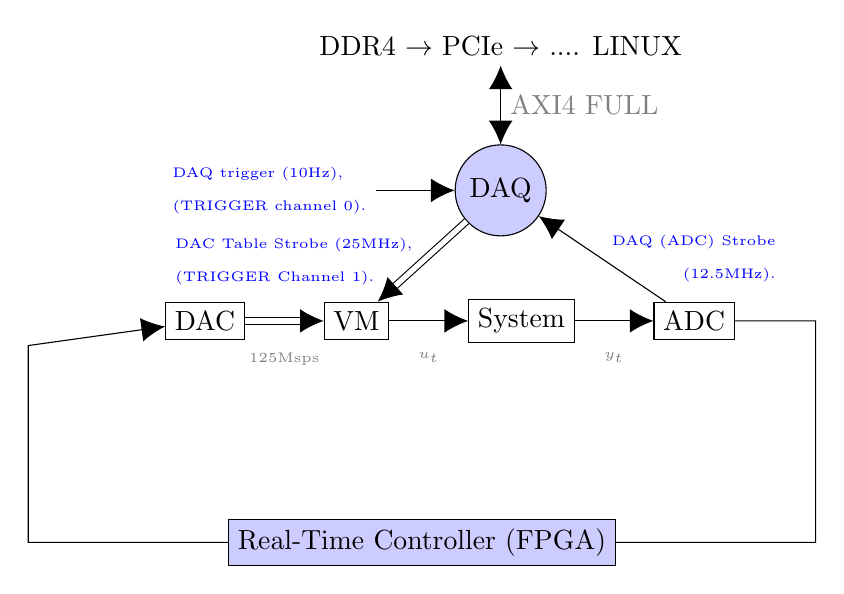
\begin{tikzpicture}
    \node (DDR) [] {DDR4 $\rightarrow$ PCIe $\rightarrow$ .... LINUX};
    \node (DAQ) [draw, circle, fill=blue!20, below=of DDR] {DAQ};
    \node (VM) [draw, below left=of DAQ] {VM};
    \node (DAC) [draw, left=of VM] {DAC};
    \node (sys) [draw,  right=of VM] {System};
    \node (ADC) [draw, right=of sys] {ADC};
    \node (n) [left=of DAQ, align=left, color=blue] {\tiny DAQ trigger (10Hz), \\ \tiny (TRIGGER channel 0).};
    
    \path [draw, <->] (DDR) -- node [right, color=gray] {AXI4 FULL } (DAQ);
    \path [draw, <-] (DAQ) -- node [right, color=blue, align=right]{\tiny DAQ (ADC) Strobe\\ \tiny (12.5MHz).} (ADC);
    \path [draw, double distance=1.9pt, ->] (DAC) -- node [color=gray, below=8.0pt] {\tiny $125$Msps} (VM);
    \path [draw, double distance=1.9pt, ->] (DAQ) -- node [left, color=blue, align=left]{\tiny DAC Table Strobe  (25MHz), \\  \tiny (TRIGGER Channel 1).} (VM);
    \path [draw, ->] (VM) -- node [color=gray, below=8.0pt] {\tiny $u_t$} (sys);
    \path [draw, ->] (sys) -- node [color=gray, below=8.0pt] {\tiny $y_t$} (ADC);
    \path [draw, ->] (ADC) -| (4,-6.3) --node [draw, fill=blue!20] {Real-Time Controller (FPGA)}  (-6,-6.3) --  (-6,-3.8) -- (DAC);
    \path [draw, ->] (n) --  (DAQ);
    \end{tikzpicture}
\end{center}



The overall architecture of the \verb|fw| VHDL code is as follows:
%\vspace{+5mm}
\begin{center}
	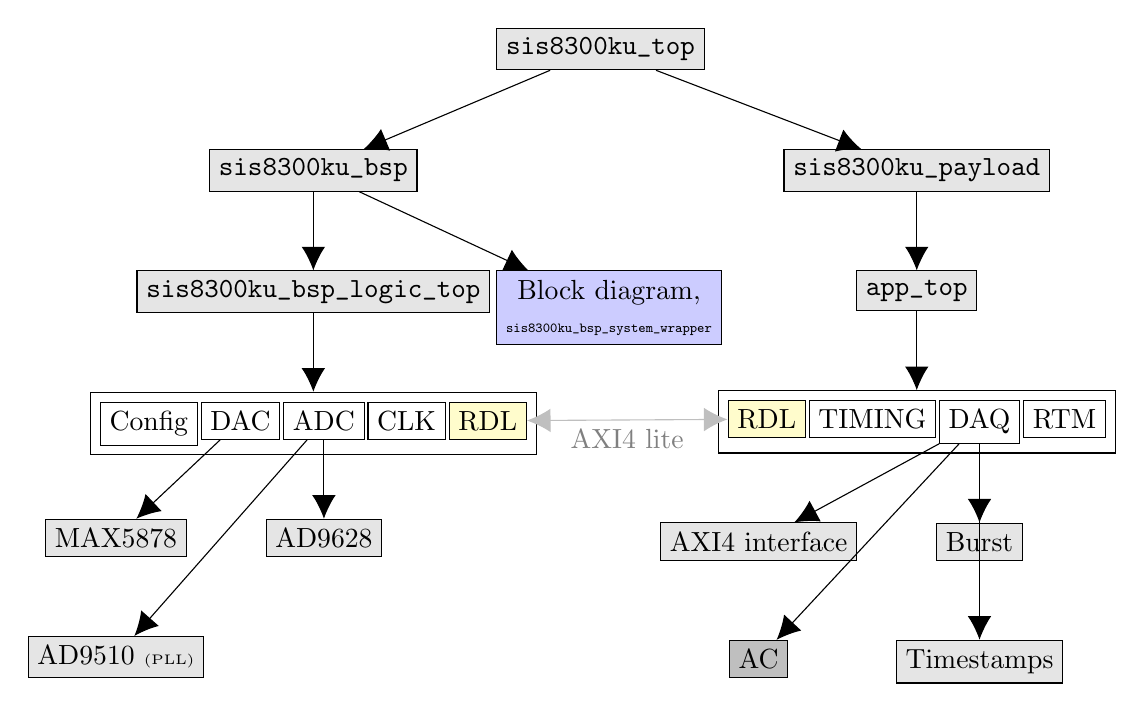
\begin{tikzpicture}
	\node (TOP) [draw, fill=gray!20] {\verb|sis8300ku_top|};
	\node (BSP) [draw, fill=gray!20,below left=of TOP] {\verb|sis8300ku_bsp|};
	\node (BD) [draw, fill=blue!20,below right=of BSP, align=center] {Block diagram,\\ {\tiny \verb|sis8300ku_bsp_system_wrapper|}};
	\node (PAY) [draw, fill=gray!20,below right=of TOP] {\verb|sis8300ku_payload|};
	\node (APP) [draw, fill=gray!20,below=of PAY] {\verb|app_top|};
	\node (L) [draw, fill=gray!20,below=of BSP] {\verb|sis8300ku_bsp_logic_top|};
	\node (LAND) [matrix, below=of L, draw, column sep=0.1em] 
	{
		\node (L10) [draw] {Config};  &
		\node (L11) [draw] {DAC}; &
		\node (L12) [draw] {ADC};  &		
		\node (L21) [draw] {CLK}; &
		\node (L22) [draw, fill=yellow!20] {RDL}; \\
	};
	\node (APPAND) [matrix, below=of APP, draw, column sep=0.1em] {
		
		\node (APP21) [draw, fill=yellow!20] {RDL}; &
		\node (APP12) [draw] {TIMING};  &
		\node (APP11) [draw] {DAQ}; &
		\node (APP22) [draw] {RTM}; \\
	};	
	\node (AD1) [fill=gray!20, draw, below=of L12] {AD9628};
	\node (MAX) [fill=gray!20, draw, left=of AD1] {MAX5878};
	\node (AD2) [fill=gray!20, draw, below=of MAX] {AD9510 {\tiny (PLL)}};
	\node (DAQ2) [fill=gray!20, draw, below=of APP11] {Burst};
	\node (DAQ1) [fill=gray!20, draw, left=of DAQ2] {AXI4 interface};
	\node (DAQ3) [fill=gray!20, draw, below=of DAQ2] {Timestamps};
	\node (AC) [fill=gray!50, draw, below=of DAQ1] {AC};
	
	\path [draw, ->] (TOP) -- (BSP);
	\path [draw, ->] (BSP) -- (BD);
	\path [draw, ->] (TOP) -- (PAY);
	\path [draw, ->] (PAY) -- (APP);
	\path [draw, ->] (BSP) -- (L);
	\path [draw, ->] (L) -- (LAND);
	\path [draw, ->] (L11) -- (MAX);
	\path [draw, ->] (L12)-- (AD1);
	\path [draw, ->] (L12)-- (AD2);
	\path [draw, ->] (APP) -- (APPAND);
	
	\path [draw, ->] (APP11) -- (DAQ1);
	\path [draw, ->] (APP11) -- (DAQ2);
	\path [draw, ->] (APP11) -- (DAQ3);
	\path [draw, ->] (APP11) -- (AC);
	
	\path [draw=gray!50,<->] (APP21) -- node [below,text=gray] {AXI4 lite} (L22); 
	\end{tikzpicture}
\end{center}


\begin{figure}[htbp] %  figure placement: here, top, bottom, or page
   \centering
   \includegraphics[width=4in]{im/schematic_dev4.png} 
   \caption{\em Schematic of the complete development. The application-specific logic resides in the {\em payload}.}
   \label{fig:schema}
\end{figure}

% desyrdl.sis8300ku_bsp_logic
% work.bsp_mmcm_wrapper
% work.app_mmcm_wrapper
% desy.app_clk_ctrl
% desy.axi4_spi_3w
% desy.clock_freq_calculator
% ADC:
%. desy.axi4_spi_3w
%. work.ent_adc_ad9628
%. 
% DAC:
%. work.ent_dac_max5878
%. 
% LED: desy.sn74lv8153
% RJ45: 
% work.fwdpga_config_manager_top

The \verb|sis8300ku_top| is tied ({\em 'constrained'}) to the pins of the FPGA in the \verb|.xdc| files.
Both AXI4 full and AXI4 light protocols are used to interconnect the involved modules,
see also  figure (\ref{fig:fwk}) and DESYs FWFWK documentation.
This design separates the development into:
\begin{itemize}
\item A hardware-specific arm (front ended by the 'board support package'), more or less tied to the hardware.
\item An application-specific arm (called the 'payload'), to be tailored to the intended application.
\end{itemize}

\begin{figure}[htbp] %  figure placement: here, top, bottom, or page
   \centering
   \includegraphics[width=4in]{im/fwfwk.png} 
   \caption{\em Overall design abstracting BSP layer from the payload (application specific) 
   	of the FWK design from DESY on which this development is based. 
	See FWK documentation.}
   \label{fig:fwk}
\end{figure}

Key top modules are:
\begin{itemize}
\item[BSP:] The Board Support Package of the SIS8300KU (Struck) card.
\item[APP:] The payload where the desired application-specific logic resides.
\end{itemize}
Key modules of the payload are:
\begin{itemize}
\item[DAQ:] The Data AcQuisition module grabbing data from the ADCs and sending those into the DDR4 using AXI4L.
\item[TIMING:] The TIMING module converts a general-purpose clock signal to trigger and strobe signals (of the DAQ).
\item[RTM:] Functionality for the RTM - in our case the DWC8VM1.
\item[RDL:] The Registers (with the RDL module describing the interface) provide the {\em glue} between the 2 arms. 
\end{itemize}
The three timing signals are as follows:
\begin{itemize}
\item[DAQ trg.:] The 10Hz trigger of the DAQ module triggers  
\item[DAC stb.:] The DAQ strobe times how fast the entries in the DAC table are fed to the DAC.
	For example, if the DAC strobe operates at 25MHz, it takes $40.96$us to realize $1024$ samples ('words') in the DAC/VM
\item[ADC stb.:] The ADC strobe (named DAQ strobe in the \verb|fw|) times the observations made from the ADCs
	and sent to the DAQ. The DAQ in turn packages those and sends the messages over AXI4 Full into the DDR4 memory.
\end{itemize}


The ADC logic works at a sampling rate of 125MS/S as follows. 
The 5 dual ADC ICs (AD9268) are driven by the clock signals generated by the 2 AD9510 PLL ICs.
 
The DAC logic works at a sampling rate of 250 MS/S.
The two digital signals (I and Q) are converted into analogue signals by DAC IC (a dual MAX 5878 ).
This signal in turn feeds a Vector Modulator (VM) IC on the RTM (the DWC8VM1 card paired with the SIS8300KU).
The resulting signal is up-converted using the LO and output at the VM output port of the RTM.
(see figure \ref{fig:card} and the manuals from the SIS8300KU and DWC8VM1).


\subsection{Memory map}

The memory map is generated and managed by desyRDL.
The description is performed in systemRDL.
The resulting map is given in .mapp files.

CERN has developed similar tools here:

\url|https://gitlab.cern.ch/be-cem-edl/common/cheby|

which interface both to the higher level control units (header files, FESA classes)
and generate source code (VHDL, ...).

\subsection{Development}

The added development in \verb|devo| is mainly invoked in the APP module. 
A convenient way to understand the development is by reading:
\begin{verbatim}
  fw > src > hw > devo > hdl > app_top.hdl
\end{verbatim}
In particular, signals \verb|pi_adc| (input signal) 
and \verb|po_dac_data_i,po_dac_data_q| (output signals) contain the 16 bit samples from the ADCs and DAC respectively.
This file also  describes instantiation of desyRDL, RTM, TIMING, DPM (dual port memory) and the DAQ module.

\subsection{Intermediate Frequency}

The intermediate frequency (IF) on which the firmware operates is set to 31.25MHz.
This means that the 125MS/S (M Samples per Second) sampler provides exactly 4 samples per cycle of the IF.
The RTM (DWC8VM1) supports a range of IF between 5MHz and 100Mhz, and we require a bandwidth of at least 20MHz.

This choice makes also a good trade-off between different effects:
\begin{itemize}
\item[(1)] We need sufficient bandwidth (and hence the IF larger than 20Mhz).
\item[(2)] We need to satisfy Nyquist: for 125MSPS, we need at most an IF=62.5MHz as we need 2 samples per cycle.

\item[(3)] Too high IF frequencies will yield considerable aliasing effects.

\item[(4)] Too low IF will result in slower artefacts because of rise time of the carrier. 
	For example, if one has an IF of 1kHz, it would take about 31 250 samples before the carrier rises to the desired maximum.

\item[(5)] Individual samples are noisy, so one likes to stay away from the bare maximal IF.
\end{itemize} 



\subsection{Latency}

The total latency of the LLRF is estimated as in table (\ref{tab:delay}).


\begin{table}
  \begin{center}
    \caption{\em Estimated latency in terms of 125 MHz (spacing 8ns) clock cycles.}
    \label{tab:delay}
    \begin{tabular}{|l || r |} % <-- Alignments: 1st column left, 2nd middle and 3rd right, with vertical lines in between
      \hline
      \textbf{Module} & \textbf{clock cycles} \\ 
      \hline
          ADC sampling	& 3 \\
       \hline
    \end{tabular}
  \end{center}
\end{table}

Latency (delay) has in general a detrimental impact on the performance (stability) of a control system,
often resulting in severe overshoot (ripple) effects.
A standard way to compensate for delay is to use a Smith control estimator.









\newpage
\addtocontents{toc}{\protect\mbox{}\protect\hrulefill\par}
\section{Digital Signal Processing}
%%%%%%%%%%%%%%%%%%%%%

\subsection{Setup}

Signals in continuous time are denoted as $y(t)$ and $u(t)$.
They are generally sampled in discrete (Zero-Order Hold, ZOH) with time constant $\tau$
and index $k$, or
\begin{equation}
	\begin{cases}
		u_k = u(k\tau) = u(t) \\
		y_k = y(k\tau) = y(t).
	\end{cases}
	\label{eq.c2d}
\end{equation}
In case of a 125 MS/S ADC sampling device, $\tau=8ns$.


\subsection{I/Q Sampling}

Consider a continuous signal $s(t)$, sampled in discrete time  $s_k$ at regular instances with $\tau>0$ spacing, or $s_k = s(k\tau)$.
This signal looks as
\begin{equation}
	s(t) = A(t) \sin\big(2\pi f_c t + \varphi(t)\big),
	\label{eq.s}
\end{equation}
with $A(t)$ denoting amplitude, and $\varphi(t)$ denoting phase.
This signal is untangled in its I-phase (I) and  In-quadrature (Q) part, denoted as $s_k^I$ and $s_k^Q$ respectively.
Both are combined into the original continuous signal $s$ as
\begin{equation}
	s(t) = I(t) \cos(2\pi f_c t) +  Q(t) \sin(2\pi f_c t),
	\label{eq.siq}
\end{equation}
or in discrete time as
\begin{equation}
	s_k = I_k \cos(2\pi f_c \tau k) +  Q_k \sin(2\pi f_c \tau k).
	\label{eq.diq}
\end{equation}
Figure (\ref{fig:iq}) displays an example of a signal with a fixed IQ value.
It follows that amplitude and phase are a nonlinear map from $I$ and $Q$ so that
\begin{equation}
	\begin{cases}
		A(t) = \sqrt{I^2(t) + Q^2(t) }\\
		\varphi(t) = \tan^{-1}\left(\frac{I(t)}{Q(t)}\right)
	\end{cases}
	\label{eq.af}
\end{equation}
and similarly in discrete time.

\begin{figure}[htbp] %  figure placement: here, top, bottom, or page
   \centering
   \includegraphics[width=5in]{im/iq.png} 
   \caption{Example of a signal with a fixed I/Q value where $I=1$ and $Q=2$.
   	In this case, we have 4 samples per cycle, and we display 4 cycles of the signal.
	If the signal has $f=125$Mhz, this would represent 128 nano seconds (i.e. $1.28e-7 s$).}
   \label{fig:iq}
\end{figure}

Fig. (\ref{fig:iq2}) gives an example of a signal with a varying IQ value:

\begin{figure}[htbp] %  figure placement: here, top, bottom, or page
   \centering
   \includegraphics[width=5in]{im/iq2.png} 
   \caption{Example of a signal with a varying I/Q value.}
   \label{fig:iq2}
\end{figure}

In general, I/Q can be recovered from $s$ as 
(see T. Schilcher, 2008, RF applications in digital signal processing, p. 257)
\begin{equation}
	\begin{cases}
		Q_k = \frac{2}{N} \sum_{l=0}^{N-1} s_{k-l} \sin\left(2\pi f_c \tau (k-l)\right) \\
		I_k = \frac{2}{N} \sum_{l=0}^{N-1} s_{k-l} \cos\left(2\pi f_c \tau (k-l)\right),
	\end{cases}
	\label{eq.neariq}
\end{equation}
where we use a least squares argument, and the quadrature property of the $\sin$ and $\cos$ parts.
This simplification relies on the assumption that the $N$ considered samples span (a number of) complete cycles of the carrier:
i.e. $N\geq 4$.
One can deviate from this restriction, but one needs then to pre-compute the (inverse of the) $cos/sin$ conversion matrices. 
Here $N$ is tuned properly.
This approach is sometimes referred to as near I/Q sampling.
In case the carrier frequency runs at 1/4 part the sampling rate (i.e. one has 4 samples per cycle of the carrier, and $N=4$),
one can simplify considerably.






\subsection{Two-sample I/Q reconstruction}

We consider an approach based on only 2 successive signal values (L. Doolittle, 2008).
This approach implies less latency, is more transparent and less reliant on the in-quadrature property,
at the price of more signal perturbation.
Assume that $I_k\approx I_{k-1}$ and $Q_k\approx Q_{k-1}$ for any $k$. 
Consider that samples $s_k$ and $s_{k-1}$ correspond with angles $t_k=k\tau$ and $t_{k-1}=(k-1)\tau$ respectively.
Then
\begin{equation}
	\begin{bmatrix}
		s_{k-1} \\
		s_{k}
	\end{bmatrix}
	=
	\begin{bmatrix}
		\cos\left(2\pi f t_{k-1} \right) &
		\sin\left(2\pi f  t_{k-1}\right) \\
		\cos\left(2\pi f t_{k}\right) &
		\sin\left(2\pi f t_{k} \right) 
	\end{bmatrix}
	\begin{bmatrix}
		I_{k-1} \\
		Q_{k-1}
	\end{bmatrix},
	\label{eq.neariqsys}
\end{equation}
or 
\begin{equation}
	\begin{bmatrix}
		I_{k-1} \\
		Q_{k-1}
	\end{bmatrix}
	= \begin{bmatrix}
		\cos\left(2\pi f t_{k-1} \right) &
		\sin\left(2\pi f  t_{k-1}\right) \\
		\cos\left(2\pi f t_{k}\right) &
		\sin\left(2\pi f t_{k} \right) 
	\end{bmatrix}^{-1}
	\begin{bmatrix}
		s_{k-1} \\
		s_{k}
	\end{bmatrix}.
	\label{eq.neariqsys2}
\end{equation}
The inverse of a $2\times 2$ matrix has a closed form solution so that 
\begin{equation}
	\begin{bmatrix}
		\cos\left(2\pi f t_{k-1} \right) &
		\sin\left(2\pi f  t_{k-1}\right) \\
		\cos\left(2\pi f t_{k}\right) &
		\sin\left(2\pi f t_{k} \right) 
	\end{bmatrix}^{-1}
	= 
	c_k
	\begin{bmatrix}
		\sin\left(2\pi f t_{k} \right) &
		- \sin\left(2\pi f  t_{k-1}\right) \\
		- \cos\left(2\pi f t_{k}\right) &
		\cos\left(2\pi f t_{k-1} \right) 
	\end{bmatrix},
	\label{eq.inv2x2}
\end{equation}
with
\begin{equation}
	c_k 
	= 
	\left(\frac{1}{\cos\left(2\pi f t_{k-1} \right) \sin\left(2\pi f t_{k} \right) 
	- \sin\left(2\pi f  t_{k-1}\right) \cos\left(2\pi f t_{k}\right)  }
	\right)
	=
	\left(\frac{1}{ \sin\left(2\pi f\tau\right) }
	\right)
	=c,
	\label{eq.inv2x2b}
\end{equation}
which is a constant independent from sampling index $k$.
This follows from a trigonometric identity.
In summary:
\begin{equation}
	\begin{cases}
		I_{k-1} = c\left( \sin\left(2\pi f t_{k} \right) s_{k-1} - \sin\left(2\pi f  t_{k-1}\right) s_{k} \right) \\
		Q_{k-1} = c\left(\cos\left(2\pi f  t_{k-1} \right) s_{k}  - \cos\left(2\pi f t_{k} \right) s_{k-1} \right),
	\end{cases}
	\label{eq.iq2}
\end{equation}
where $c$ is a constant.
In case $f\tau=\frac{1}{4}$, traditional I/Q sampling is recovered and $c=1$.

\begin{figure}[htbp] %  figure placement: here, top, bottom, or page
   \centering
   \includegraphics[width=5in]{im/iq3.png} 
   \caption{\em Example of a signal with a varying I/Q value where I/Q is recovered via above argument.
   Here white noise with a SNR of 10 is added to the samples.}
   \label{fig:iq3}
\end{figure}

%
%\begin{tikzpicture}
%\draw (-1.5,0) -- (1.5,0);
%\draw (0,-1.5) -- (0,1.5);
%\draw (0,0) circle [radius = 1cm];
%\end{tikzpicture}


%
%In simple terms, we denote this conversion in terms of a matrix:
%\begin{equation}
%	u_k 
%	= u_k^I \cos \left( 2\pi\frac{f_c}{f_S} k \right)
%	+ u_k^Q \sin\left(2\pi\frac{f_c}{f_S} k \right)
%	= \IM_k
%	\begin{bmatrix}
%		u_k^I \\
%		u_k^Q
%	\end{bmatrix},
%	\label{eq.ADCd_iqu}
%\end{equation}
%where
%\begin{equation}
%	\IM_k
%	=
%	\begin{bmatrix}
%		\cos \left( 2\pi\frac{f_c}{f_S} k \right) &
%		\sin\left(2\pi\frac{f_c}{f_S} k \right)
%	\end{bmatrix}\in\R^{1\times 2}.
%	\label{eq.ADCd_iqy}
%\end{equation}
%

\subsection{Synchronization}
%%%%%%%%%%%%%%%%




In our particular case, the pulses will be fed with a carrier having a various initial phase offset.
Figure (\ref{fig:pulsex}) displays an example of two sampled pulses with 4s between, 
as sampled using exactly the same hardware/firmware settings. Note that the initial phase offset is adrift.
This means e.g. that full IQ sampling (hitting the cycle at phase {\em exactly} equal to $0,\frac{\pi}{2}, \pi, \frac{3\pi}{2}$) is not going to work.



\begin{figure}[htbp] %  figure placement: here, top, bottom, or page
   \centering
   \includegraphics[width=2in]{im/pulse1.png} 
   \includegraphics[width=2in]{im/pulse2.png} 
   \caption{\em Two readings of a pulse 4s apart.
   	Note that the 'small signal' before the actual pulse (a delay of 28 samples) is due to path mismatching.}
   \label{fig:pulsex}
\end{figure}


However, the REF signal provides a reliable signal absolutely stable across pulses.
That means that when a pulse trigger comes, the value of the REF signal indicates the phase of the carrier at that instance.
This value can then be used to compensate the phase offset by rotating the carrier accordingly.
We describe below how this works.

Rather than performing this explicitly, we integrate this phase offset compensation within our 2sample reconstruction scheme.
It is convenient to use complex notation with $\Re(\cdot)$ representing the real part, and $\Im(\cdot)$ the imaginary part of its argument. 
In this case, the signal is represented as 
\begin{equation}
	s(t) = \Re\left( e^{j \omega t + j\phi}\right) = \Re\left( e^{j\phi} \ e^{j \omega t}\right).
	\label{eq.csignal}
\end{equation}
Comparison to the IQ representation of equation (\ref{eq.siq}) gives 
\begin{equation}
	\begin{cases}
		 Q(t) = \Re\left( e^{j  \phi}\right) \\
		  I(t) = - \Im\left( e^{j  \phi}\right),
	\end{cases}
	\label{eq.csignal2iq}
\end{equation}
as $\Re\left( e^{j \omega t}\right) = \cos(\omega t)$ and the in-quadrature $\Im\left( e^{j \omega t}\right) = \sin(\omega t)$, and from the rules of multiplication of complex numbers 
$(a+jb)(c+jd)=(ac-bd) + j (ad+bc)$.
Now, let $\phi_i$ denote the random phase offset of pulse $i$.
Since $\sin\left(\theta-\frac{\pi}{2}\right)= - \cos(\theta)$
or $\Im(e^{j\theta}) = - \Re\left(e^{j\left(\theta-\frac{\pi}{2}\right)}\right)$, 
it follows that the I and Q values according to the random phase offset are given as
\begin{equation}
	I(\phi_i) 
	= - \Im\left( e^{j  \phi_i}\right) 
	= \Re\left( e^{j\phi_i - j\frac{\pi}{2}}\right) 
	= \Re\left( e^{ - j\frac{\pi}{2}} \ e^{j\phi_i}\right), 
	\label{eq.csignal.offset}
\end{equation}
and assuming a sampling rate of $4\omega$ gives $I_k = Q_{k-1}$.
Assume that we have a reference signal $r$ with constant $I$ and $Q$ values. 
This then implies that a signal with a random phase offset of every pulse 
can be tied to this $r$ by compensating the observed IQ values of the
observed signal with $r_k$ and $r_{k-1}$ respectively. 


In practice, we can observe the reference signal 
\begin{equation}
	r(t) = \Re\left( e^{j\omega t} \right),
	\label{eq.csignal.r}
\end{equation}
with unspecified initial condition $t=0$.
We also observe the relevant signal as 
\begin{equation}
	s(t) = \Re\left( e^{j\omega t + j m(t)}\right). 
	\label{eq.csignal.r}
\end{equation}
with $m$ denoting the relevant information as modulated on the carrier.
The question now reads as how to find the compensated signal $s^c$ defined as 
\begin{equation}
	s^c(t)  = \Re\left( e^{j\omega (t-t_i) + j m(t)}\right) = \Re\left( e^{-j\omega t_i} \ e^{j\omega t + j m(t)}\right), 
	\label{eq.csignal.sc}
\end{equation}
with $t_i$ indicating the time the $i$th pulse starts.
Expanding this product gives 
\begin{multline}
	s^c(t)  
	= \Re\left( e^{j\omega t + j m(t)}\right) \  \Re\left( e^{-j\omega t_i}\right) -  \Im\left( e^{j\omega t + j m(t)}\right)\ \Im\left( e^{-j\omega t_i}\right) \\
	= \Re\left( e^{j\omega t + j m(t)}\right) \  \Re\left( e^{-j\omega t_i}\right) +  \Im\left( e^{j\omega t + j m(t)}\right)\ \Im\left( e^{j\omega t_i}\right) \\
	= r(t_i) s(t) \  + \ {r}\left(t_i-\frac{\pi\omega}{2}\right) s\left( t-\frac{\pi\omega}{2}\right).
	\label{eq.csignal.sc2}
\end{multline}
Note that this expression relies {\em not} on any particular frequency or sampling rate.
On the other hand, if the sampling rate were exactly $4\frac{\omega}{2\pi}$, the discrete time version becomes 
\begin{equation}
	s^c_k
	= r(t_i) s_k \  + \ {r}\left(t_i-\frac{\pi\omega}{2}\right) s_{k-1},
	\label{eq.csignal.sc3}
\end{equation}
as before.


\newpage
\addtocontents{toc}{\protect\mbox{}\protect\hrulefill\par}
\section{Mathematical models and descriptions}
%%%%%%%%%%%%%%%%%%%%%%%%

\subsection{Pulse compressor}

Any cavity of a pulse compressor is adequately described as 
an inductor, a capacitor and a resistor (LCR) circuit (Woolley and Syratchev, 2017).
The voltage equals the real part of the complex-valued function $V$, which solves 
\begin{equation}
	\frac{1}{L} \int V(t) dt + C\dfrac{dV(t)}{dt} + \left(\frac{1}{R_s} + \frac{1}{Z_{wg}}\right) V(t)
	= 
	\frac{2F}{Z_{wg}} e^{j\omega t},
	\label{eq.lcr}
\end{equation}
where $Z_{wg}$ is the impedance of the transmission line into the cavity,
$R_s$ is the cavity shunt impedance,
and $F$ is the phasor of the forward wave into the cavity.
The phasor $F$ is typically given by the application.
The phasor $R$ of the outgoing wave at the port of the cavity is determined as the solution to 
\begin{equation}
	V(t) = \left(F(t) + R(t)\right) e^{j\omega t}
	\label{eq.lcr2}
\end{equation}
The outgoing wave is the sum of reflected and emitted wave.

\begin{figure}[htbp] %  figure placement: here, top, bottom, or page
   \centering
   \includegraphics[width=3in]{im/pc2.png} 
   \caption{\em Schematic layout of a SLED-I pulse compressor.}
   \label{fig:pc2}
\end{figure}

Using reparameterisations  
\begin{equation}
	\begin{cases}
		\omega_0 = \frac{1}{\sqrt{LC}} \\
		Q_0 = \omega_0 R_s C \\
		\frac{1}{Q_L} = \frac{1}{Q_0} + \frac{1}{Q_e}, 
	\end{cases}
	\label{eq.lcr1b}
\end{equation}
one gets the more familiar 2e order system description
\begin{equation}
	\dfrac{d^2 V(t)}{ dt^2} 
	+ \left(\frac{\omega_0}{Q_L}\right)\dfrac{dV(t)}{ dt} 
	+ \omega_0^2 V(t)
	=
	\left(\frac{2\omega_0}{Q_e}\right) \dfrac{d}{dt} \left(F(t) e^{j\omega t}\right).
	\label{eq.lcr3}
\end{equation}
with $F$ the phasor describing the input signal.

\subsection{Waveguide}

A waveguide guides an electromagnetic wave over a distance in a material.
Description starts with the wave equation for electric field $E(t)$ given as 
\begin{equation}
	c_0^{-2} \dfrac{\partial^2 E(t)}{\partial t^2} - \nabla^2 E(t) = 0,
	\label{eq.wave}
\end{equation}
where $c_0=2.998\times 10^8$ for vacuum (or $c_0 = 1/\sqrt{\mu\epsilon}$ otherwise, 
with permeability $\mu$ and permittivity $\epsilon$ of the material inside the waveguide).


%\url{https://phys.libretexts.org/Bookshelves/Electricity_and_Magnetism/Book%3A_Electromagnetics_II_(Ellingson)/06%3A_Waveguides/6.08%3A_Rectangular_Waveguide-_TM_Modes}


\subsection{SSPA}

Figure (\ref{fig:sspa}) displays a first characterisation of the S-band power amplifier.

\begin{figure}[htbp] %  figure placement: here, top, bottom, or page
   \centering
   \includegraphics[width=2in]{im/sspa4.png} 
   \includegraphics[width=2in]{im/sspa3.png} \\
   \includegraphics[width=2in]{im/sspa1.png} 
   \includegraphics[width=2in]{im/sspa2.png} 
   \caption{\em Characterisation of the solid state power amplifier (SSPA) for the S-band (3GHz).
   (a) $P_{in} - P_{out}$ characterisation of the SSPA (without pre-driver).
   (b) PA element.
   (c) Layout (including the pre-driver embedding).
   (d) Schematic.}
   \label{fig:sspa}
\end{figure}

\subsection{Klystron+K100}



(ScandiNova) Klystron based RF unit. 
Designed to provide RF peak power in the 3 MW to 10 MW range, it provides unparalleled performance and ease of integration and use by customers. 
Can be provided as a pure pulse modulator all the way to turn-key RF System. Below are specifications and data sheets for the most common configurations based on frequency and type of klystron.


\begin{table}
	\begin{center}
	\begin{tabular}{r|l}\hline\hline
	RF peak power		& 3 – 10 MW \\
	RF average power 	& 10 kW (max)\\
	Pulse voltage		& 115 – 190 kV\\
	Pulse current		& 90 – 140 A\\
	\hline
   \end{tabular}
   \caption{Specifications of the K100 pulse modulator (Scandinova), powered by a Klystron vacuum tube.}
  \end{center}
\end{table}


\newpage
\addtocontents{toc}{\protect\mbox{}\protect\hrulefill\par}
\section{Automatic control algorithms}
%%%%%%%%%%%%%%%%%%%%


The general control loop looks as follows:

\begin{center}
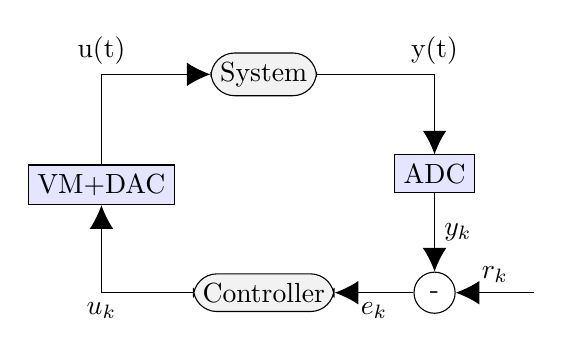
\begin{tikzpicture}
\node (S) [draw, fill=gray!10, rounded corners=3mm] {System};
\node (center) [below=of S] {};
\node (C) [draw, , fill=gray!10, below=of center, rounded corners=3mm] {Controller};
\node (VM) [left=of center, draw, fill=blue!10] {VM+DAC};
\node (-) [right=of C, circle,draw] {-};
\node (ADC) [above=of -, draw, fill=blue!10] {ADC};
\node (c) [right=of -] {};

\path [draw, ->] (ADC) -- node [auto] {$y_k$} (-);
\path [draw,->] (-) -- node [below] {$e_k$} (C);
\path [draw, ->] (C) -| node [below] {$u_k$} (VM);
\path [draw, ->] (VM) |- node [above] {u(t)} (S);
\path [draw, ->] (S) -| node [above] {y(t)}(ADC);
\path [draw, ->] (c) -- node [above] {$r_k$} (-);
\end{tikzpicture}
\end{center}
From the above discussion, we see that there are 6 output signals $y(t)$, while there is only a single input signal $u(t)$.
For the single input single output (SISO) control loops, we work only with the output signal on BC2.fwd (see Fig. (\ref{fig:loop1})).

There are two main effects:
\begin{itemize}
\item[FF] Repeatable pulse-to-pulse disturbances are handled by feedforward (FF) control.
\item[FB] Non-repeating external disturbances (on the flat-top of the pulse) are handled by feedBack (FB) control.
\end{itemize}
In the present context, it is convenient to represent the reference signal $r_k$ as a trigger signal.
Three events are announced in this trigger signal:
\begin{itemize}
\item Start filling the RF field - a new pulse is coming in 15us! 
\item Realise the pulse now!
\item Reverse phase for the pulse compressor!
\end{itemize}
see also figure (\ref{fig:pulse}.b).




\subsection{PID Control Loops}
%%%%%%%%%%%%%%%%



The de facto standard approach is to implement two independent PI(D) loops on the I and the Q branch of the signal.
The PID control loop is a SISO loop, meaning it can only handle a single input and single output signal.
In this case, we use as input the VM driving the SSPA, and as output signal the reading from BC4.fwd. 
This SISO loop is shown in figure (\ref{fig:loop2}).

\begin{figure}[htbp] %  figure placement: here, top, bottom, or page
   \centering
   \includegraphics[width=5in]{im/loop1.png} 
   \caption{\em Layout of the SISO control loops implemented by a PID controller on both I and Q arms.}
   \label{fig:loop2}
\end{figure}

The common design is to have independent  I and Q  arms, denoted respectively as $C^I$ and $C^Q$:
For the control of a single resonating cavity, this design is close to optimal (O. Troeng 2019). 

\begin{center}
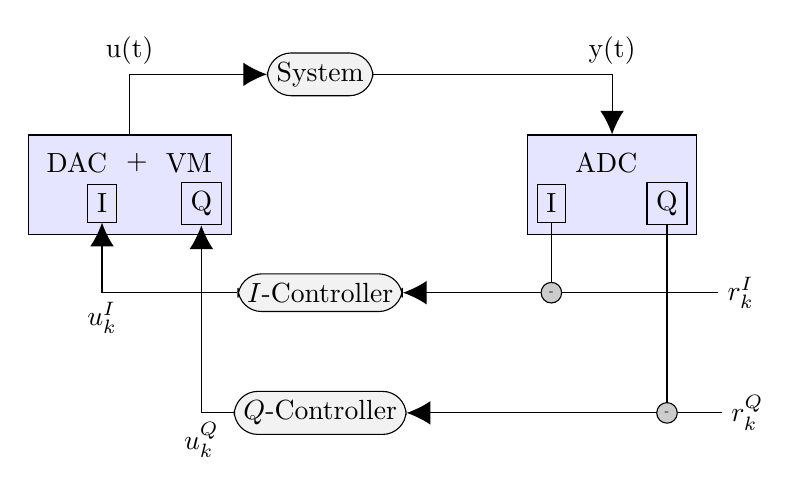
\begin{tikzpicture}
\node (S) [draw, fill=gray!10, rounded corners=3mm] {System};
\node (center) [below=of S] {};
\node (CI) [draw, , fill=gray!10, below=of center, rounded corners=3mm] {$I$-Controller};
\node (CQ) [draw, , fill=gray!10, below=of CI, rounded corners=3mm] {$Q$-Controller};
\node (VM) [matrix,left=of center, draw, fill=blue!10] {
	\node (VM11) {DAC}; &
	\node (VM12) {+}; &
	\node (VM13) {VM}; \\
	\node (VM21) [draw]{I}; &
	\node (VM22) [] {}; &
	\node (VM23) [draw] {Q}; \\};
\node (ADC) [matrix,right=2.5cm of center, draw, fill=blue!10] {
	\node (ADC11) {}; &
	\node (ADC12) {ADC}; &
	\node (ADC13) {}; \\
	\node (ADC21) [draw] {I}; &
	\node (ADC22) {   }; &
	\node (ADC23) [draw] {Q}; \\};
\node (rq) [right=4cm of CQ] {$r_k^Q$};
\node (ri) [right=4cm of CI] {$r_k^I$};

\path [draw, ->] (ADC21) |- node (I-) [circle, scale=0.5, draw,fill=gray!40] {-} (CI);
\path [draw, ->] (ADC23) |-  node (Q-) [circle, scale=0.5, draw,fill=gray!40] {-} (CQ);

\path [draw, ->] (CI) -| node [below] {$u^{I}_k$} (VM21);
\path [draw, ->] (CQ) -| node [below] {$u^{Q}_k$} (VM23);
\path [draw, ->] (VM) |- node [above] {u(t)} (S);
\path [draw, ->] (S) -| node [above] {y(t)}(ADC);
\path [draw] (ri) --  (I-);
\path [draw] (rq) --  (Q-);
\end{tikzpicture}
\end{center}
or
\begin{equation}
u_k = C^I\left( r_k^I - I_k\right) \cos\left(2\pi f_c \frac{k}{f_S}\right) 
	+ C^Q\left( r_k^Q - Q_k\right) \sin\left(2\pi f_c \frac{k}{f_S}\right).
\label{eq.pidiq}
\end{equation}
Since the control blocks can implement phase shift (delay), independence of the I and Q paths is not necessary preserved.
That is, the same output behaviour can be achieved using different controller settings, resulting in ill conditioning of the problem.

Let's focus now on a single arm (say, the I-arm).
The PID loop is described by the following equations.
A continuous version of a PID loop is given as 
\begin{equation}
	u(t) = K_p e(t) + K_i \int_0^t e(\tau) d\tau + P_d \left(\dfrac{de(t)}{dt}\right),
	\label{eq:piBC}
\end{equation}
where 
\begin{equation}
	e(t) = r(t) - y(t), \ \forall t,
	\label{eq:piBCe}
\end{equation}
and $T_p,T_i,T_d\geq 0$ are parameters to be tuned. 
A discretised version of a PID loop is given as 
\begin{equation}
	u_k = u_{k-1} + P_0 e_{k-1} + P_2 e_{k-2} + P_2 e_{k-3},
	\label{eq:pid}
\end{equation}
where 
\begin{equation}
	e_k = r_k - y_k, \ \forall k,
	\label{eq:pid}
\end{equation}
and $P_0, P_1, P_2$ are equivalent parameters to be tuned 
(i.e. there exists a one-to-one mapping from $P_p, P_i, P_d$ to $P_0, P_1, P_2$
depending on the used discretisation scheme).

\subsection{Anti-windup filter}

Anti-windup filters provide a standard way to handle saturation effects for avoiding overly large integrator terms.
An implementation of the familiar Smith anti-windup approach is included in the firmware.

%\subsection{Ripple filter}
%
%(To be specified)

\subsection{Feedforward Tables}

A considerable control effort is implemented in a feedforward way - i.e. in a pulse-to-pulse way.
Especially, the EM field is build up by implementing pre-recorded actions when needed.
That is, if the bunch pre-warning messages arrives,  this table will be implemented at $u$.
FeedBack serves as an add-on to handle non-repetitive (stochastic) noise/disruptions.

A pulse of 6 us spans 750 samples (at 125 MS/S).
A filling of 600 ns spans an extra 75 samples.
So a pulse is spanned well by a sequence of 1024 samples, starting roughly 1us in advance.
 
The setup of a feedforward (FF) controller is displayed below.
Here, the real-time controller is denoted as $C$.
The system to be controlled is denoted as $P$ ('Plant'), mapping
input $u_k$ to output $y_k$. There is no {\em direct} feedBack in this case.

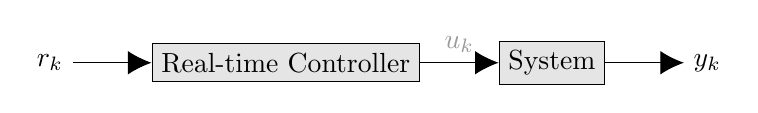
\begin{tikzpicture}
\node (C) [draw, fill=gray!20] {Real-time Controller};
\node (P) [draw, right=of C, fill=gray!20] {System};
\node (r) [left=of C] {$r_k$};
\node (y) [right=of P] {$y_k$};
\path [draw, ->] (C) -- node [above, color=gray!80] {$u_k$} (P);
\path [draw, ->] (r) -- (C);
\path [draw, ->] (P) -- (y);
\end{tikzpicture}

However, in the present case it is more convenient to represent FF control as a table of values to be 
injected when a new pulse will be made (at 10Hz).


\subsection{Iterative Learning Control}

The feedforward table are adjusted by an adaptive pulse-to-pulse scheme.
This scheme corresponds roughly to iterative learning control (ILC).
Let $[k]$ denote the pulse iteration of sample $k$.
That is, if the iteration takes $n>0$ samples, then $[k]= \lfloor \frac{k}{n}\rfloor$ (also referred as the quotient).
The remainder is given as $(k) = k \mbox{ \ mod \ } n$, indicating the index in the present 
iteration to which the $k$th sample relates.
For example, let an iteration be spanned by $n=10$ samples. Then sample $k=25$ would fall in the $[k]=2$e iteration, 
on the $(k)=5$e place within this 2e iteration. 

Then the main ILC approach can be denoted as 
\begin{equation}
	u_{[k],(k)} = u_{[k]-1, (k)} + \fbox{$P_0 e_{[k]-1,(k)} +  P_1 e_{[k]-2,(k)} +  P_2 e_{[k]-3,(k)}$}.
	\label{eq.ilc}
\end{equation}
Here, the content of the framed box indicates the {\em update} of the feedforward table from the previous pulse.
In case of a fixed number of $n$ samples in an iteration, one has 
\begin{equation}
		\begin{cases}
			u_{s,i} = u_{ns+i}\\
			e_{s,i} = r_{ns+i} - y_{ns+i},
		\end{cases}
	\label{eq.ilc2}
\end{equation}
where $s$ indexes {\em iteration}, and $i$ the {\em sample} in this iteration.
Again, $P_0,P_1,P_2$ are to be tuned properly.

% 
%It will be convenient to include the ADC+VM+DAC in the system, so that the following block diagram holds for either the I or Q arm:
%
%\begin{center}
%\begin{tikzpicture}[point/.style={circle,inner sep=0pt,minimum size=2pt,fill=white}]
%\node (S) [draw, fill=gray!10, matrix,column sep=2mm] {
%\node (VM) [draw, fill=blue!10] {VM};
%& \node (DAC) [draw, rounded corners=3mm, fill=blue!10] {DAC};
%& \node (Sys) [draw, rounded corners=3mm,fill=white] {System};
%& \node (ADC) [draw, rounded corners=3mm, fill=blue!10]  {ADC}; \\
%};
%\node (center) [below=of ADC] {};
%\node (C) [draw, , fill=gray!10, below=of center, rounded corners=3mm] {Controller};
%\node (L) [draw,point,left=of S] {};
%\node (-) [draw,right=of C,circle] {-};
%\node (ref) [right=of -] {$r_k$};
%
%\path [draw] (C) -| (L);
%\path [draw,->] (L) -- node [above] {$u_k$} (VM);
%\path [draw] (C) -- (-);
%\path [draw,->] (ADC) -| node [above] {$y_k$} (-);
%\path [draw,->] (-) -- node [above] {$e_k$} (C);
%\path [draw, ->] (ref) -- (-);
%
%\path [draw] (VM) -- (DAC) -- (Sys) -- (ADC);
%\end{tikzpicture}
%\end{center}
%
%The dynamical discrete-time system $u_k \rightarrow y_k$ is described for any $k$ as
%\begin{equation}
%\begin{cases}
%\begin{bmatrix}
%x_{k+1,1} \\
%x_{k+1,2} \\
%x_{k+1,3} \\
%x_{k+1,4}
%\end{bmatrix}
%=
%\AM
%\begin{bmatrix}
%x_{k,1} \\
%x_{k,2} \\
%x_{k,3} \\
%x_{k,4}
%\end{bmatrix}
%+
%\BM u_k
%\\ \ \ \ \ \
%\begin{bmatrix}
%y_k^I \\
%y_k^Q
%\end{bmatrix}
%=
%\CM
%\begin{bmatrix}
%x_{k,1} \\
%x_{k,2} \\
%x_{k,3} \\
%x_{k,4}
%\end{bmatrix}
%+
%\DM u_k
%\end{cases}
%\label{eq.ADCd}
%\end{equation}
%with $\AM\in\R^{4\times 4}$ defined as
%\begin{equation}
%\AM
%=
%\begin{bmatrix}
%a_{11} & a_{12} & a_{13}  & a_{14} \\
%a_{21} & a_{22} & a_{23} & a_{24}  \\
%a_{31} & a_{32} & a_{33} & a_{34}\\
%a_{41} & a_{42} & a_{43} & a_{44} \\
%\end{bmatrix}
%\label{eq.ADCd_iqu}
%\end{equation}
%and $\BM\in\R^{4\times 2}$ as
%\begin{equation}
%\BM
%=
%\begin{bmatrix}
%b_{11} & b_{12} \\
%b_{21} & b_{22} \\
%b_{31} & b_{32}   \\
%b_{41} & b_{42} \\
%\end{bmatrix}
%\label{eq.ADCd_iqu}
%\end{equation}



\newpage
\addtocontents{toc}{\protect\mbox{}\protect\hrulefill\par}
\section{Control firmware}
%%%%%%%%%%%%%%%%%

\subsection{Control loop}

As indicated before, the control loop implements the stages as displayed in Figure (\ref{fig:func2}):
\begin{figure}[htbp] %  figure placement: here, top, bottom, or page
   \centering
   \includegraphics[height=2.5in]{im/loop2023.png} 
   \includegraphics[height=1in]{im/firmware.png} 
   \caption{\em Schematic overview of the implemented feedback loop.}
   \label{fig:func2}
\end{figure}
The key idea is to separate within-pulse and pulse-to-pulse components out of the signal $s$.
Then, either component is addressed with their appropriate feedback loop.
\begin{figure}[htbp] %  figure placement: here, top, bottom, or page
   \centering
   \includegraphics[height=2.5in]{im/pulsedsignal.png} 
   \caption{\em A regularly pulsed signal (left panel) can be folded in a multivariate fashion in Pulse-to-Pulse and within-pulse dimensions (right panel).}
   \label{fig:pulsed}
\end{figure}


\subsubsection{Within-Pulse feedback}
%%%%%%%%%%%%%%%%%%%%


\subsubsection{Pulse-to-Pulse feedback}
%%%%%%%%%%%%%%%%%%%%%

\section{Numerical representation}

We use 64 bit fixed point numerical representations, with the final result truncated to 16 (15+1) bit integers.
The fixed point representation is $s32.32$, or 
1 sign bit (2-complement), 32 integer bits, and $32$ fractional bits. 
There are at least three good reasons for this decision:
\begin{itemize}
\item Future DACs will have a resolution exceeding the current 16 bit, but we like the development to handle those cases seamlessly.
\item Since the loops are fairly complex, numerical errors will accumulate quickly.
\item We like to be fairly robust towards changing dynamical range.
\end{itemize}
The firmware developments on top of the BSP consists of the following modules ('IP cores').

\section{IP cores}
%%%%%%%%%%

\subsection{IQ demodulation core}

\begin{figure}[htbp] %  figure placement: here, top, bottom, or page
   \centering
   \includegraphics[width=2in]{im/IQcore.png} 
   \caption{Overview of the I/Q demodulation core.}
   \label{fig:iqcore}
\end{figure}

\subsection{Rotation core}


\begin{figure}[htbp] %  figure placement: here, top, bottom, or page
   \centering
   \includegraphics[width=2in]{im/ROTcore.png} 
   \caption{Overview of the core implementing a rotation table.}
   \label{fig:rotcore}
\end{figure}



\subsection{IIR filter core}

\begin{figure}[htbp] %  figure placement: here, top, bottom, or page
   \centering
   \includegraphics[width=2in]{im/IIRcore.png} 
   \caption{Overview of the  core realising an Infinite Impulse Response (IIR) filter.}
   \label{fig:iircore}
\end{figure}



\subsection{ILC Control core}

\begin{figure}[htbp] %  figure placement: here, top, bottom, or page
   \centering
   \includegraphics[width=2in]{im/ILCcore.png} 
   \caption{Overview of the core implementing the Iterative Learning Control (ILC) pulse-to-pulse control loop.}
   \label{fig:ilccore}
\end{figure}


\subsection{PID core}


\begin{figure}[htbp] %  figure placement: here, top, bottom, or page
   \centering
   \includegraphics[width=2in]{im/PIDcore.png} 
   \caption{Overview of the core implementing a PID feedback control loop}
   \label{fig:pidcore}
\end{figure}




















\newpage
\addtocontents{toc}{\protect\mbox{}\protect\hrulefill\par}
\section{Graphical User Interface}
%%%%%%%%%%%%%%%%%

The central way to interact with this firmware is through a graphical user interface (GUI) connected to the COMex and the firmware
via PCI express. This interface allows to get all samples from the DAQ (via Direct Memory Access, or DMA), and to change settings in the memory map.
A key design decision is to wait for explicit events (click on 'Update!') for acquiring new signals to be fed to the GUI:
there is no continuous event system as to keep the GUI lightweight.

Figure (\ref{fig:gui}) displays an example of a 5MHz carrier signal, where 25 samples are made per cycle.
The GUI shows the 8 channels for a fixed pair SIS8300ku+DWC8VM1 in a specified slot of the crate.
Since the software is run on the COMex (MCH-RTM), the selection of card need only be made on the software side (in the according .dmap file).

\begin{figure}[htbp] %  figure placement: here, top, bottom, or page
   \centering
   \includegraphics[width=4in]{im/gui2.png} 
   \caption{\em The GUI developed to monitor and setup the firmware project.}
   \label{fig:gui}
\end{figure}



\subsection{Software interface to firmware}

The high-level (but slow) software is run on the COMex (Python3.8.10 on Ubuntu 20.04 TLS, running on Xeon on the MCH-RTM), accepting information (of the DAQ) 
via PCI express. The interface is served by the package mtca4u.py, which is a Python wrapper of the DESY-developed framework.
%
%
%\subsection{Calibration}
%
%\subsection{Settings}
%
%\subsubsection{Setting clocks}
%\subsubsection{Setting interrupts (IRQs)}
%\subsubsection{Setting interlocks (IRKs)}
%\subsubsection{Channel-specific settings}
%
%



\newpage
\addtocontents{toc}{\protect\mbox{}\protect\hrulefill\par}
\section{Conclusion}
%%%%%%%%%%%

This development implements a low level (LLRF) control system for use in a plasma-driven particle accelerator (AWAKE) project in CERN.
The development uses the MicroTCA hardware, and builds further on the framework developed by DESY.
Practical operation of the development is enabled via a GUI (written in Python), running on the linux system integrated in the MicroTCA crate on the rear 
(MCH-RTM).  The aim is to integrate this LLRF system in the overall supervisory control (SCADA) framework as used in CERN (i.e. the socalled FESA system) 
or as used elsewhere (e.g EPICS).

\section{Research challenges}
%%%%%%%%%%%%%%%%

\begin{itemize}
\item Pulsed Control is a fascinating, and underdeveloped control paradigm. 
         The approach taken here - integrating feedback schemes with pulse-to-pulse (learning) control,
         provides a practical solution but is riddled by lacking theoretical understanding.
         Especially questions regarding long-term control stability of the integrated system are wide open.
         However, since the system at hand is fast but simple (second order), those questions do not imply any practical challenges as yet. 
          
\item Fast ADC: it is possible to achieve effectively high sampling rates ($>$1GSPS) by using a suitable combination of slow, cheap ADC sampling hardware.
	This is know as the emerging paradigm of 'sub-Nyquist' sampling.
	The most direct way is to use interleaving ADC samplers, providing "only" a linear increase.
	For example, interleaving 4 ADCs of 125MSPS will give one effective fast ADC of 500 MSPS.
	This enables direct sampling (DS) mechanisms, rather than the need to down convert the signals to lower frequencies (IF) with implied constraint bandwidths.
\end{itemize}


\end{document}